\pdfminorversion=4
\documentclass[]{beamer}
%for printing or having a crappy pdf reader backup
%\documentclass[handout]{beamer}
\mode<presentation>
\usetheme{Madrid}
\usecolortheme[RGB={80,0,0}]{structure}
%teal \usecolortheme[RGB={0,128,128}]{structure}
\useoutertheme{miniframes}
\useinnertheme{default}
\usepackage{color}
\definecolor{Maroon}{RGB}{80,0,0}
\definecolor{BurntOrange}{RGB}{204,85,0}
\usepackage{setspace}
\usepackage{amsmath}
\usepackage{amsthm}
\usepackage{amsfonts}
\usepackage{amssymb}
\usepackage{verbatim}
\usepackage{array}
\usepackage{graphicx}
\usepackage{subfigure}
\usepackage{colortbl}
%\usepackage[retainorgcmds]{IEEEtrantools}
\usepackage{wrapfig}
\usepackage[figurename=,tablename=]{caption}
\usepackage{multirow}
\usepackage{bm}
\setbeamercolor{normal text}{fg=black}
\setbeamercovered{dynamic}
\beamertemplatetransparentcovereddynamicmedium
%\usepackage{chronology}
\setbeamertemplate{caption}[numbered]
\usepackage{colortbl}
\newcommand {\mathsym}[1]{{}}
\newcommand {\unicode}{{}}
\newcommand{\om}{\boldsymbol{\Omega}}
\newcommand{\etal}{{\it et al.\,}}
\newcommand{\vr}{\vec{r}}
\newcommand{\vo}{\vec{\Omega}}
\newcolumntype{L}{>{\centering\arraybackslash}m{3cm}}
\newcommand{\tcr}[1]{\textcolor{red}{#1}}
%Creating a norm command
\newcommand{\norm}[1]{\left\lVert#1\right\rVert}
%Allow page breaks within align
\allowdisplaybreaks
%Code
\usepackage{listings}
\usepackage{pdfpages}
\newlength \figwidth
\setlength \figwidth {0.5\textwidth}

%Hyperlinking
\usepackage{hyperref}


\begin{document}
%	
\title[GitHub Tutorial]{Basic GitHub Tutorial}
\author[Ghaddar]{Tarek Habib Ghaddar}
\institute[TAMU]{Nuclear Engineering \\ CLASS \\ Texas A\&M University}
\date[March 30, 2018]

{
\setbeamertemplate{headline}[default] 
\begin{frame}
\vspace{-1.1cm}
	\begin{figure}[t]
		\centering
			
\includegraphics[width=.25\textwidth]{figures/seal.png}
	\end{figure}
\vspace{-0.75cm}
\titlepage
\end{frame}
}

\begin{frame}
\tableofcontents
\end{frame}

\section{Introduction}
\subsection{}
\begin{frame}[t]\frametitle{Background}
  \begin{block}{Why Version Control?}
    \begin{itemize}
      \item Keeps a software system consisting of many versions and configurations well organized.
      \item Allows everyone to see what changes are being made.
      \item Offers a back up in case of destroyed hard drive, weird wipe, act of God, etc..
    \end{itemize}
  \end{block}
\end{frame}

\begin{frame}[t]\frametitle{Background}
  \begin{block}{Git Vs. GitHub}
    \begin{itemize}
      \item Git is the version control software, GitHub is the interface.
    \end{itemize}
  \end{block}
  \begin{block}{GitHub at TAMU}
  \begin{itemize}
    \item TAMU offers a free enterprise account to students, faculty, etc.
    \item Just login with your TAMU NetID and password to GitHub Enterprise.
    \item Allows you to make repository private for free.
    \item \url{https://github.tamu.edu}
  \end{itemize}
\end{block}
\end{frame}

\section{Getting Started}
\subsection{}

\begin{frame}[t]\frametitle{GitHub Desktop}
\begin{block}{}
\begin{itemize}
  \item A nice, easy to use, GUI that walks the user through some of the some slightly complex parts of GitHub.
  \item Does not have the power/fidelity of the terminal interface.
  \item \url{https://desktop.github.com}
\end{itemize}
\end{block}
\end{frame}

\begin{frame}
\centering
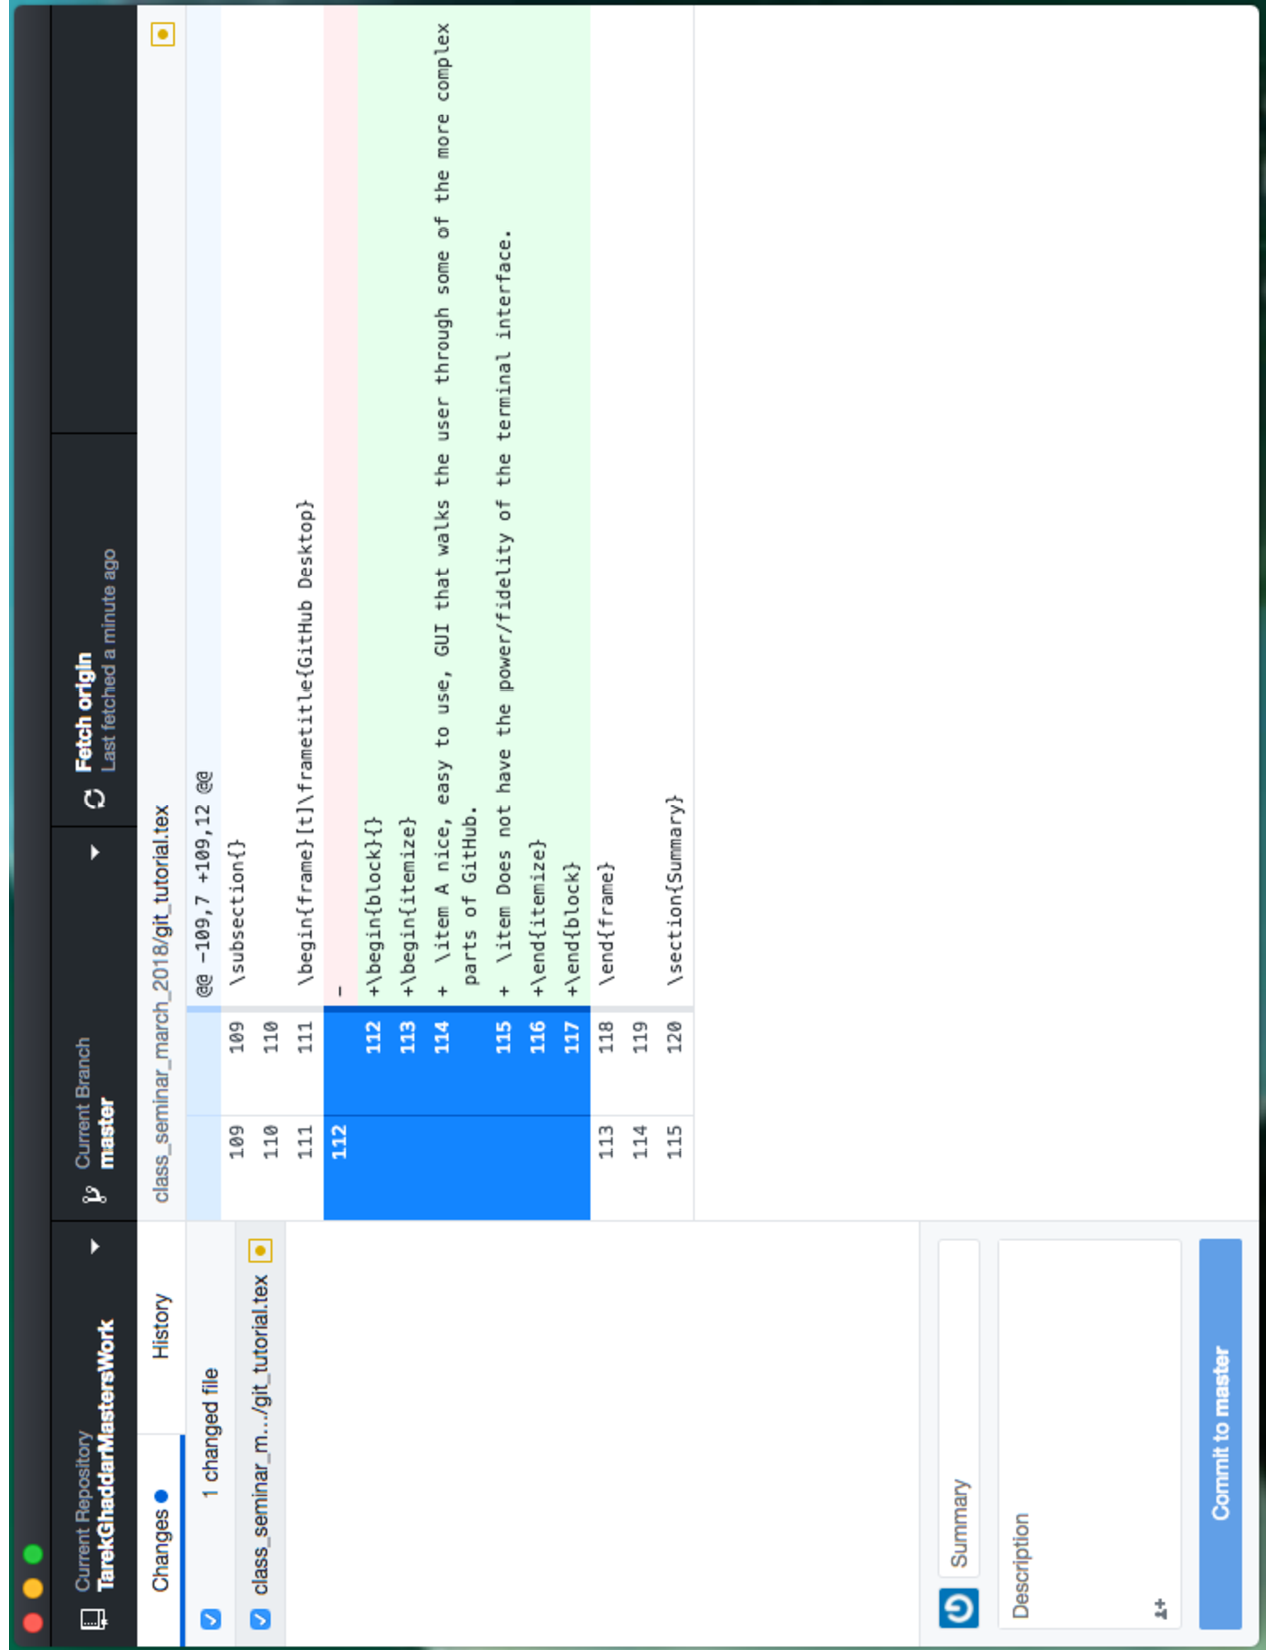
\includegraphics[scale=0.39,angle=-90,origin=c]{figures/desktop_0.pdf}
\end{frame}

\begin{frame}
\centering
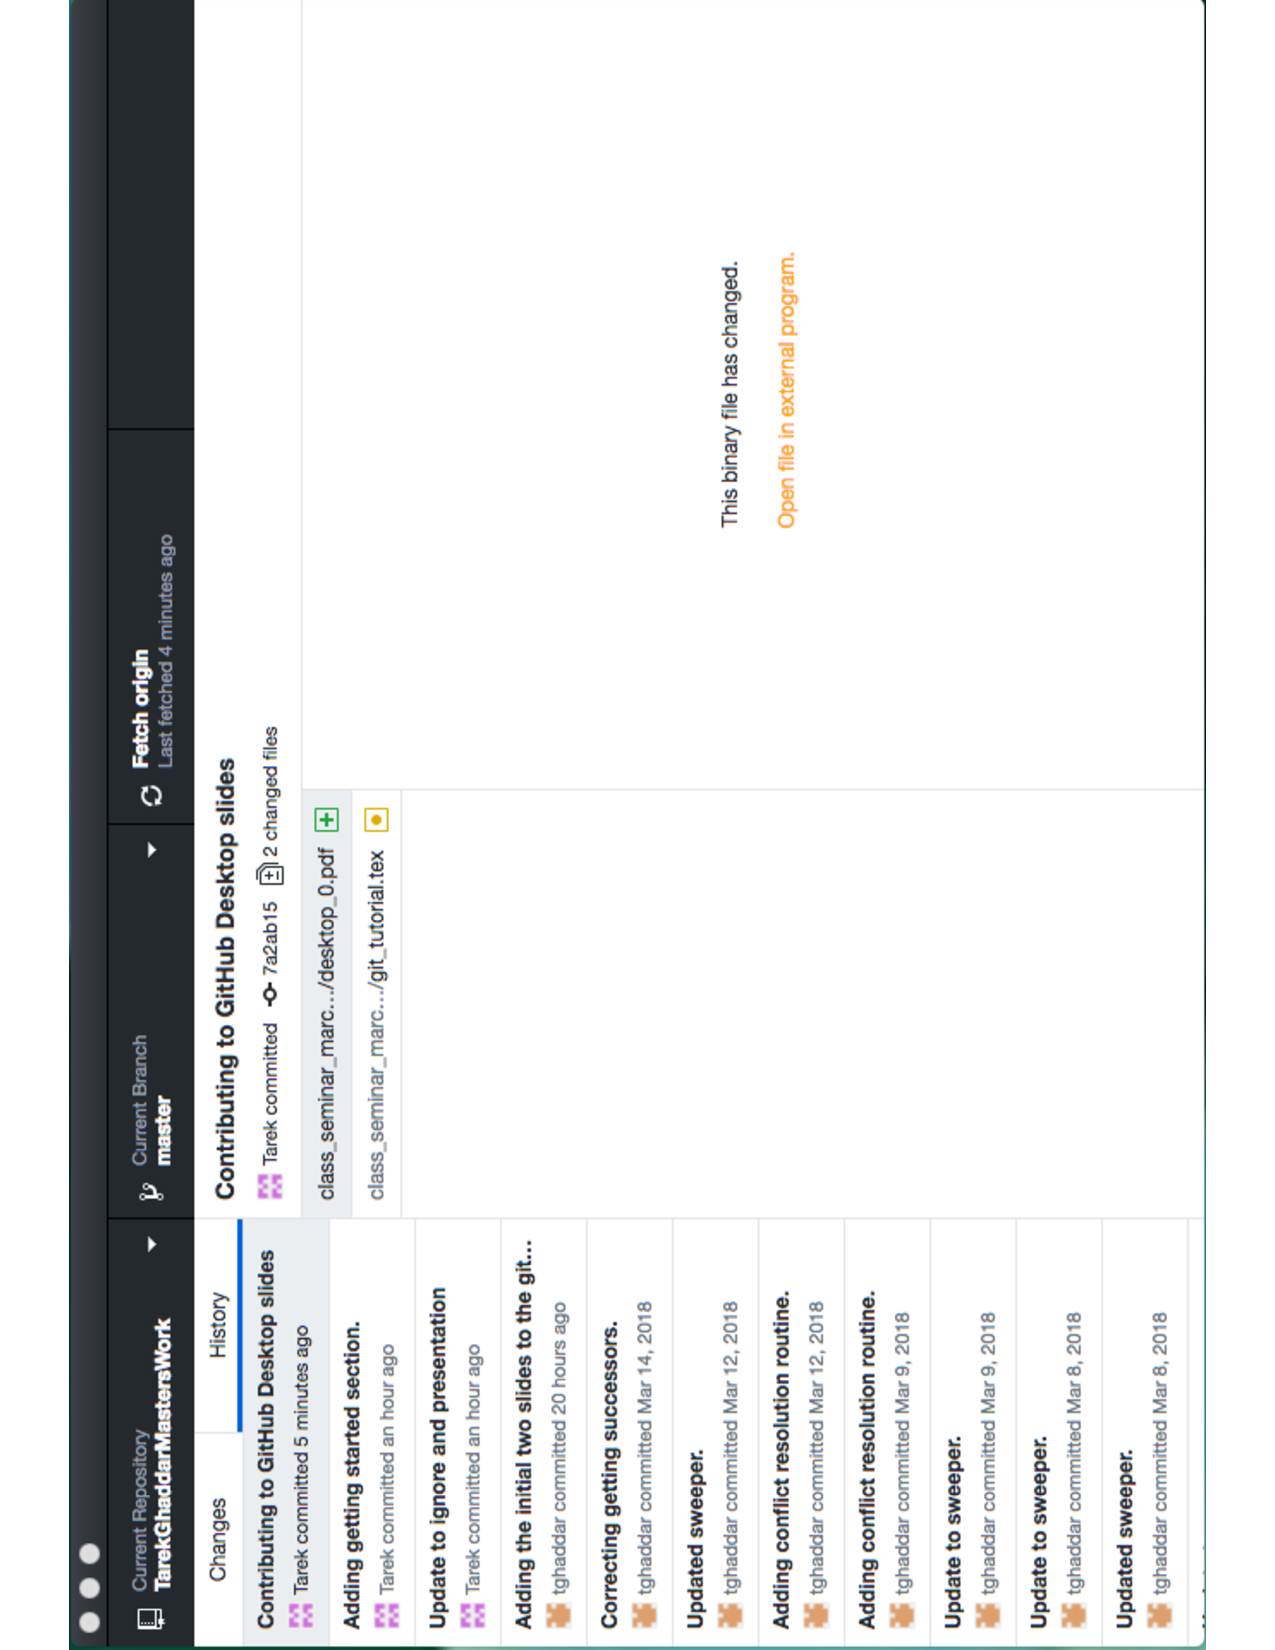
\includegraphics[scale=0.39,angle=-90,origin=c]{figures/desktop_history.pdf}
\end{frame}

\section{Important Files and Commands}

\subsection{Files}
\begin{frame}[t]\frametitle{.gitingore File}
\centering
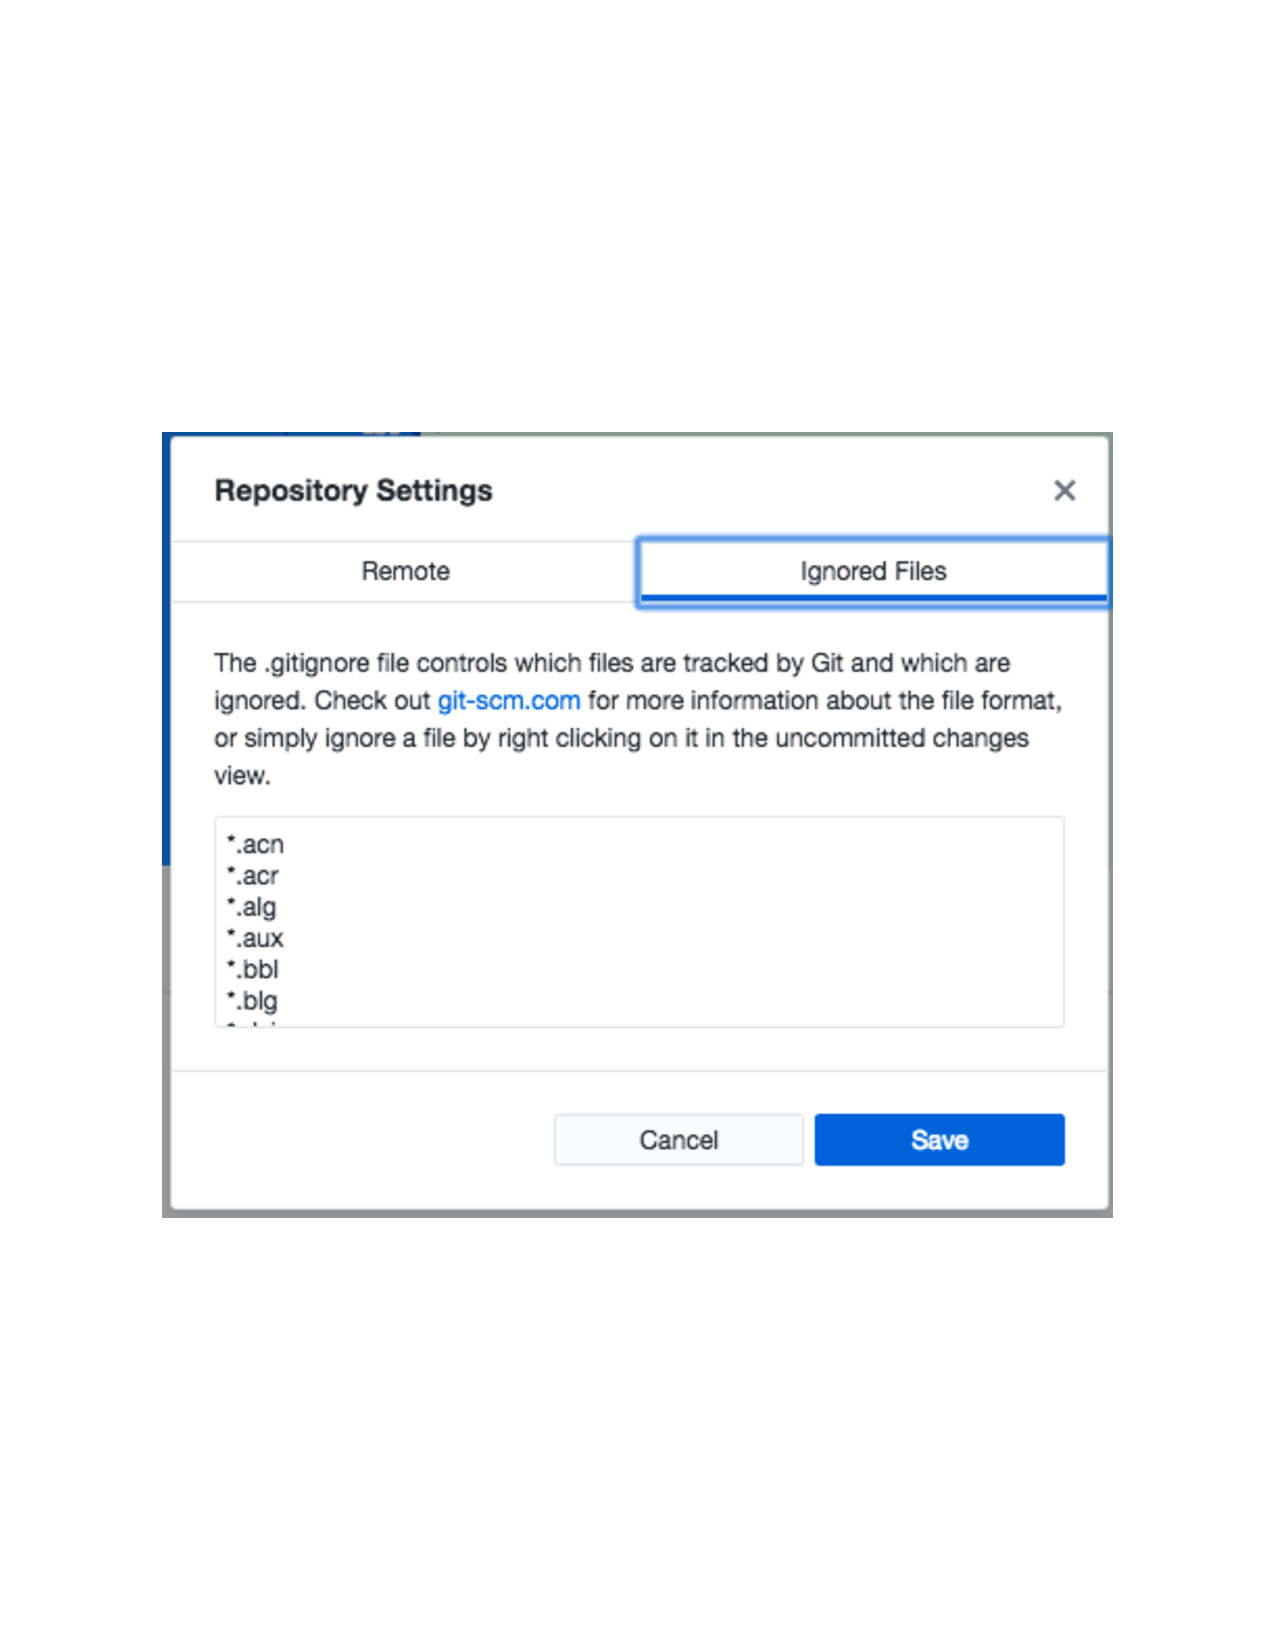
\includegraphics[scale = 0.49, trim={1.06in 2.83in 1.05in 2.84in},clip]{figures/gitignore_image.pdf}
\end{frame}

\subsection{Commands}
\begin{frame}[t]\frametitle{Commit/git commit}
\begin{columns}
\begin{column}{.6\textwidth}
\begin{block}{} 
\begin{itemize}
  \item A user commits to their local copy of their repository. 
  \item This DOES NOT update the remote (online) repository.
  \item Your commit is a local, offline, ``save point" in your repository.
  \end{itemize}
\end{block}
\end{column}

\begin{column}{0.38\textwidth}
\centering
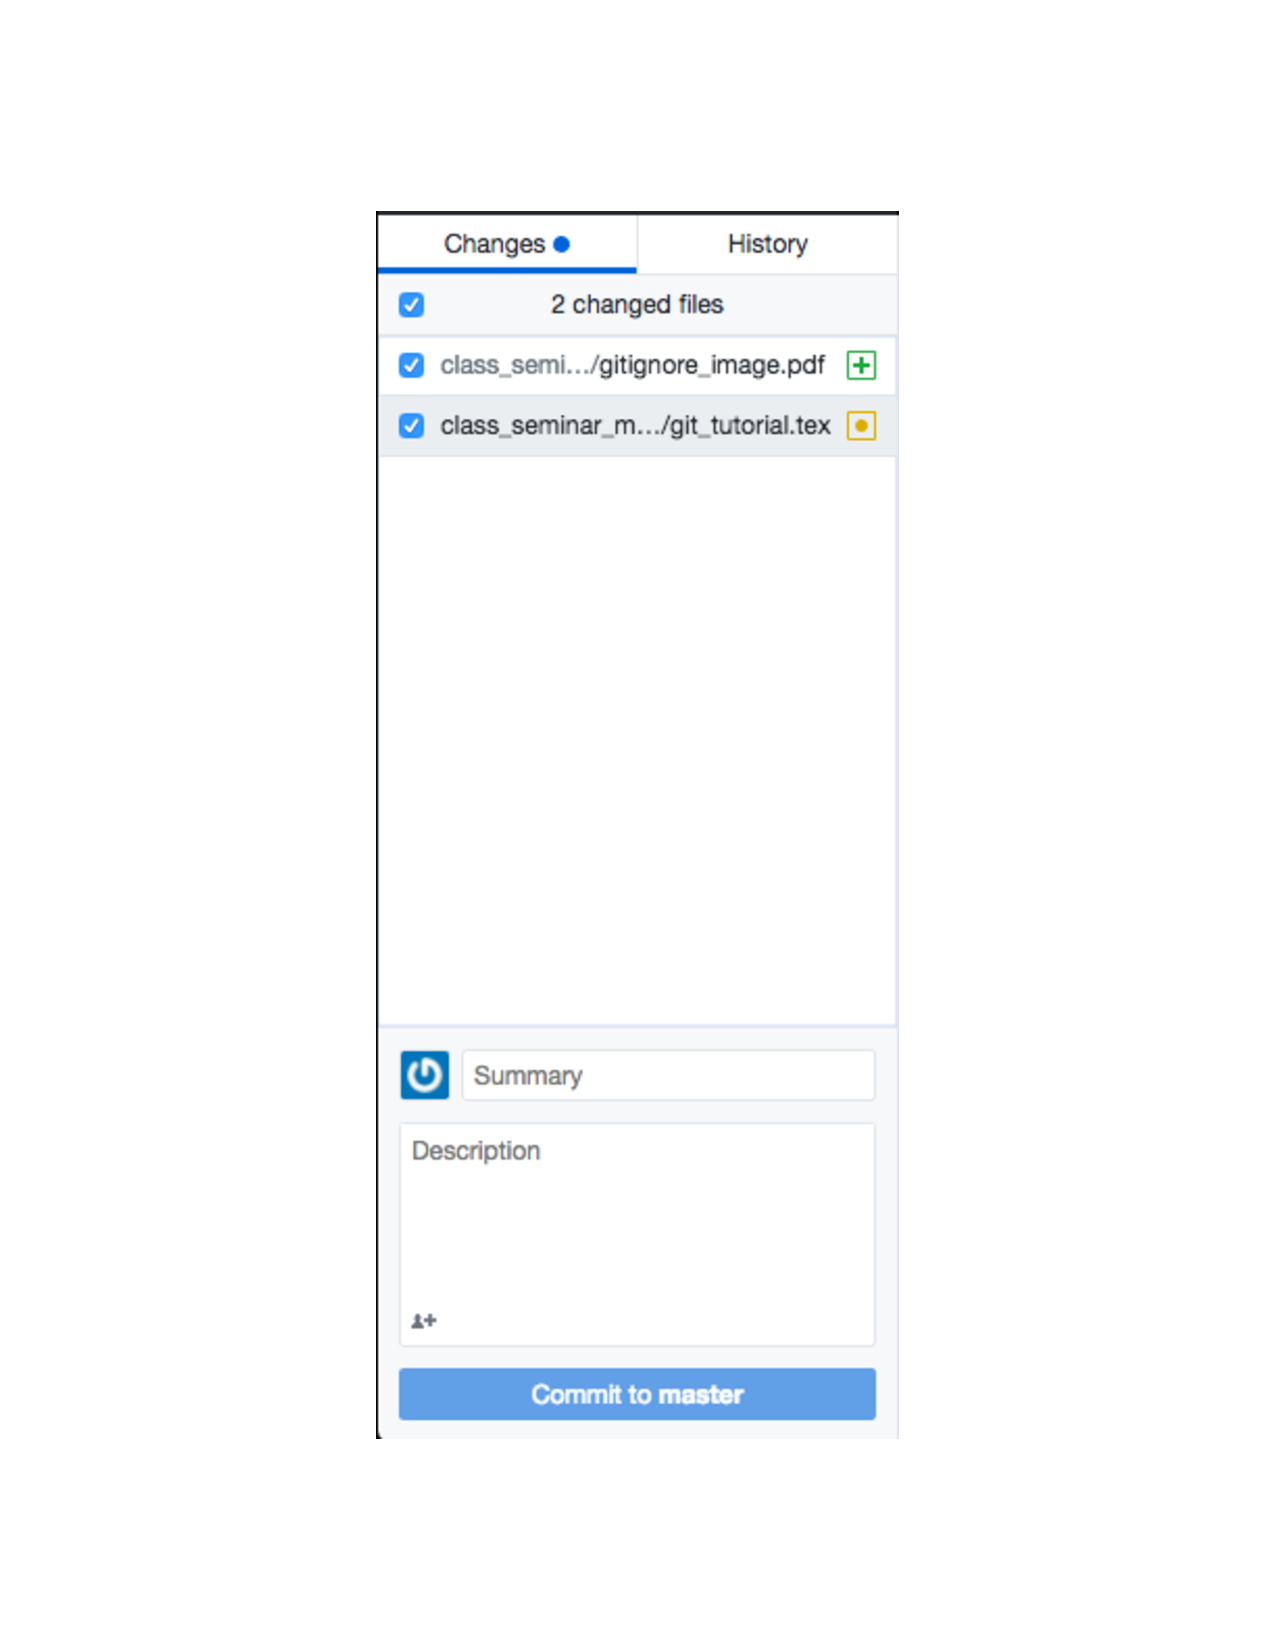
\includegraphics[scale = 0.30,trim={2.49in 1.39in 2.49in 1.39in},clip]{figures/commit_image.pdf}
\end{column}
\end{columns}

\end{frame}

\section{Branches, Forks, and Pull Requests}
\subsection{}

\begin{frame}[t]{Forking a Repository}

\end{frame}

\section{Summary}
\subsection{}
\begin{frame}[t]\frametitle{Best Practices}
  \begin{block}{}
    \begin{enumerate}
      \item ALWAYS pull in changes from the online repository before working on your local copy. 
        \begin{itemize}
          \item Version Control Maxim: "He who commits first, wins."
        \end{itemize}
      \item If there is a conflict, merge your changes responsibly.
      \item ALWAYS make sure your code compiles and runs before committing and pushing.
      \item NEVER push binary files, executables, or large files. 
      \item If you don't know what to do, ask someone more knowledgeable, or check StackOverflow and similar sites.
    \end{enumerate}
  \end{block}
\end{frame}


\end{document}
